% \documentclass[aspectratio=169,notes]{beamer}
\documentclass[aspectratio=169]{beamer}
\usetheme[faculty=phil]{fibeamer}
\usepackage{polyglossia}
\setmainlanguage{english} %% main locale instead of `english`, you
%% can typeset the presentation in either Czech or Slovak,
%% respectively.
\setotherlanguages{russian} %% The additional keys allow
%%
%%   \begin{otherlanguage}{czech}   ... \end{otherlanguage}
%%   \begin{otherlanguage}{slovak}  ... \end{otherlanguage}
%%
%% These macros specify information about the presentation
\title[AGLA1]{Analytical Geometry and Linear Algebra I, Lab 11} %% that will be typeset on the
\subtitle{Affine Transformation
\\ \   \\ \ 
         } %% title page.
\author{Oleg Bulichev}
%% These additional packages are used within the document:
\usepackage{ragged2e}  % `\justifying` text
\usepackage{booktabs}  % Tables
\usepackage{tabularx}
\usepackage{tikz}      % Diagrams
\usetikzlibrary{calc, shapes, backgrounds}
\usepackage{amsmath, amssymb}
\usepackage{url}       % `\url`s
\usepackage{listings}  % Code listings
% \usepackage{subfigure}
\usepackage{floatrow}
\usepackage{subcaption}
\usepackage{mathtools}
\usepackage{todonotes}
\usepackage{fontspec}
\usepackage{multicol}
\usepackage{pdfpages}
\usepackage{wrapfig}
\usepackage{animate}
\usepackage{booktabs}
\usepackage{multirow}

\graphicspath{{resources/}}
\frenchspacing

\setbeamertemplate{caption}[numbered]
\usetikzlibrary{graphs}

% \usepackage[backend=biber,style=ieee,autocite=footnote]{biblatex}
% \addbibresource{biblio.bib}
% \DefineBibliographyStrings{english}{%
%   bibliography = {References},}

\newcommand{\oleg}[2][] {\todo[color=red, #1] {OLEG:\\ #2}}
\newcommand{\fbckg}[1]{\usebackgroundtemplate{\includegraphics[width=\paperwidth]{#1}}}%frame background

\usepackage[framemethod=TikZ]{mdframed}
\newcommand{\dbox}[1]{
\begin{mdframed}[roundcorner=3pt, backgroundcolor=yellow, linewidth=0]
\vspace{1mm}
{#1}
\vspace{1mm}
\end{mdframed}
}

\begin{document}
\setlength{\abovedisplayskip}{0pt}
\setlength{\belowdisplayskip}{0pt}
\setlength{\abovedisplayshortskip}{0pt}
\setlength{\belowdisplayshortskip}{0pt}

\fbckg{fibeamer/figs/title_page.png}
\frame[c]{\setcounter{framenumber}{0}
    \usebeamerfont{title}%
    \usebeamercolor[fg]{title}%
    \begin{minipage}[b][6.5\baselineskip][b]{\textwidth}%
        \textcolor{black}{\raggedright\inserttitle}
    \end{minipage}
    % \vskip-1.5\baselineskip

    \usebeamerfont{subtitle}%
    \usebeamercolor[fg]{framesubtitle}%
    \begin{minipage}[b][3\baselineskip][b]{\textwidth}
        \raggedright%
        \insertsubtitle%
    \end{minipage}
    \vskip.25\baselineskip
}
%   \frame[c]{\maketitle}

\fbckg{fibeamer/figs/common.png}

\note{Решения к ответам лежат в отдельной папке}
% \begin{frame}[t]{Questions for today}
%     \framesubtitle{}
%     \begin{itemize}
%         \item How can I work with general form of 2nd order curve equation?
%         \item How it relates with cone?
%         \item What forms of equation do we have?
%     \end{itemize}
% \end{frame}

\begin{frame}[t]{Affine Transformation}
\framesubtitle{Formal definition}
\textbf{Classical representation}:\smallskip
    \begin{align*}
        \begin{bmatrix}x^*\\y^*\end{bmatrix} = \begin{bmatrix}
        a & b\\ 
        c & d 
        \end{bmatrix}\begin{bmatrix}x\\y\end{bmatrix} + \begin{bmatrix}x_0\\y_0\end{bmatrix}
    \end{align*} 

    \textbf{System of equations representation}:\smallskip
    \begin{align*}
        \left\{\begin{matrix*}[l]
        x^*=ax+by+x_0\\
        y^*=cx+dy+y_0 
        \end{matrix*}\right.
    \end{align*}
    \textbf{Homogeneous representation}:\smallskip
    \begin{align*}
        \begin{bmatrix}x^*\\y^*\\1\end{bmatrix}=\begin{bmatrix}
        a & b & x_0 \\
        c & d & y_0 \\ 
        0 & 0  & 1 
        \end{bmatrix}\begin{bmatrix}x\\y\\1\end{bmatrix}
    \end{align*}
\end{frame}

\begin{frame}[t]{Affine Transformation}
    \framesubtitle{Video: formal definition}
    \vspace{-0.6cm}
    \begin{figure}[H]
        \href{https://www.youtube.com/watch?v=il6Z5LCykZk}{
            \centering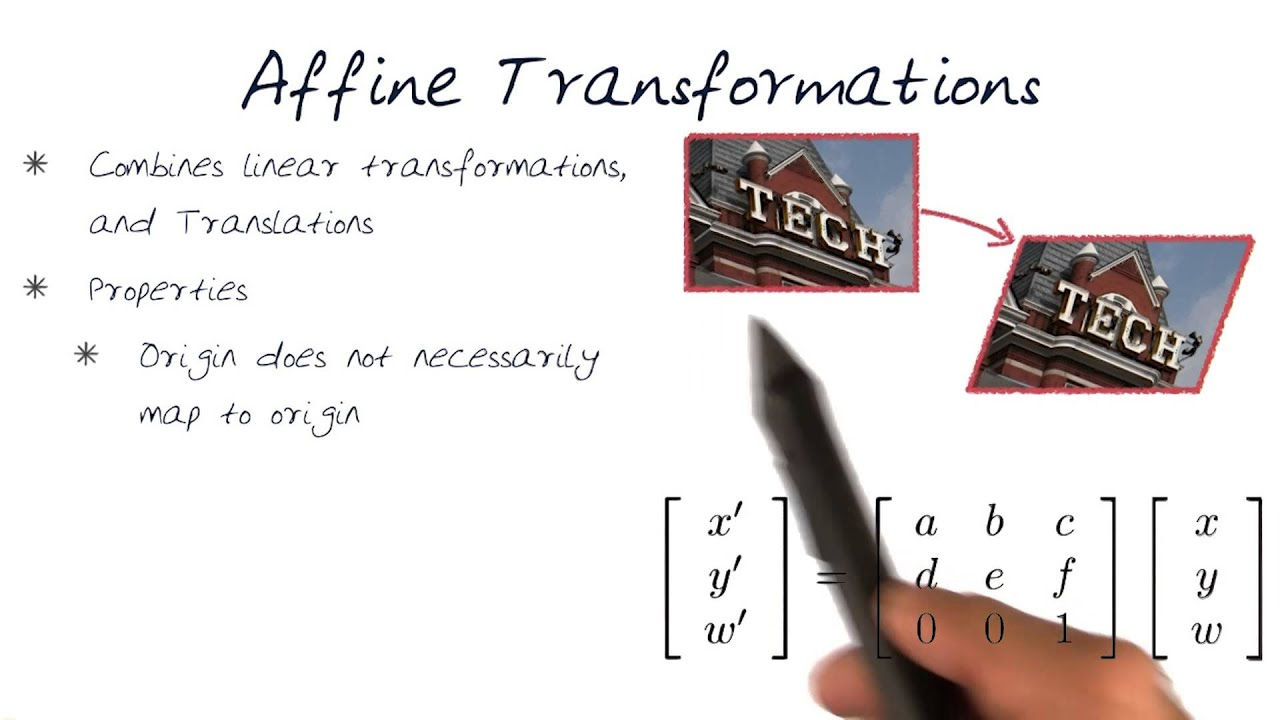
\includegraphics[height=6cm,width=1\textwidth,keepaspectratio]{formal_def.jpg}}
        % \caption{Click on a picture for a video}
        \label{fig:formal_def.jpg}
    \end{figure}
\end{frame}

\begin{frame}[t]{Affine Transformation}
    \framesubtitle{Porperties}
        \begin{itemize}
            \item \textit{Collinearity between points}: three or more points which lie on the same line (called collinear points) continue to be collinear after the transformation.
            \item \textit{Parallelism}: two or more lines which are parallel, continue to be parallel after the transformation.
            \item \textit{Convexity of sets}: a convex set continues to be convex after the transformation. Moreover, the extreme points of the original set are mapped to the extreme points of the transformed set.
            \item \textit{Ratios of lengths} of parallel line segments are the same after the transformation.
        \end{itemize}
    \end{frame}

\begin{frame}[t]{Task 1}
    \framesubtitle{}
    Linear transformation of a real axis is given by $f(x)=ax+b$. (a) Find all fixed points of this transformation. (b) Find the transformation that is inverse for $f$.

    \uncover<2->{
        \alert{\Large Answer}

        (a) If $a\neq1$ then there is one fixed point $x=\dfrac b{1-a}$; if $a=1$ and $b=0$ then all points are fixed; if $a=1$ and $b\neq0$ then there are no fixed points. (b) It exists only if $a\neq0$: $f^{-1}(y)=\dfrac{y-b}a$.
    }
\end{frame}

\begin{frame}[t]{Task 2}
    \framesubtitle{}
    An affine transformation is given by $x^*=3x+2y-6$, $y^*=4x-3y+1$. Find the images of (a) point $M(-1;\,5)$; (b) line $2x+3y=7$.

    \uncover<2->{
        \alert{\Large Answer}

        (a) $(1;-18)$\\ (b) $18x-5y-6=0$.
    }
\end{frame}




\begin{frame}[t]{Task 3}
    \framesubtitle{}
    Two linear transformations of a real axis $f$ and $g$ are given by $f(x)=ax+b$, $g(x)=cx+d$. Find compositions of transformations $fg$ and $gf$. What are the necessary and sufficient conditions for $fg$ to be equal to $gf$?
    
    \uncover<2->{
        \alert{\Large Answer}
        
        $(fg)(x)=acx+ad+b$; $(gf)(x)=acx+bc+d$; $fg=gf\Leftrightarrow d(a-1)=b(c-1)$.
    }
\end{frame}

% \begin{frame}[t]{Bijection, injection and surjection}
% \framesubtitle{}
%     \vspace{-0.6cm}
%     \begin{figure}[H]
%         \centering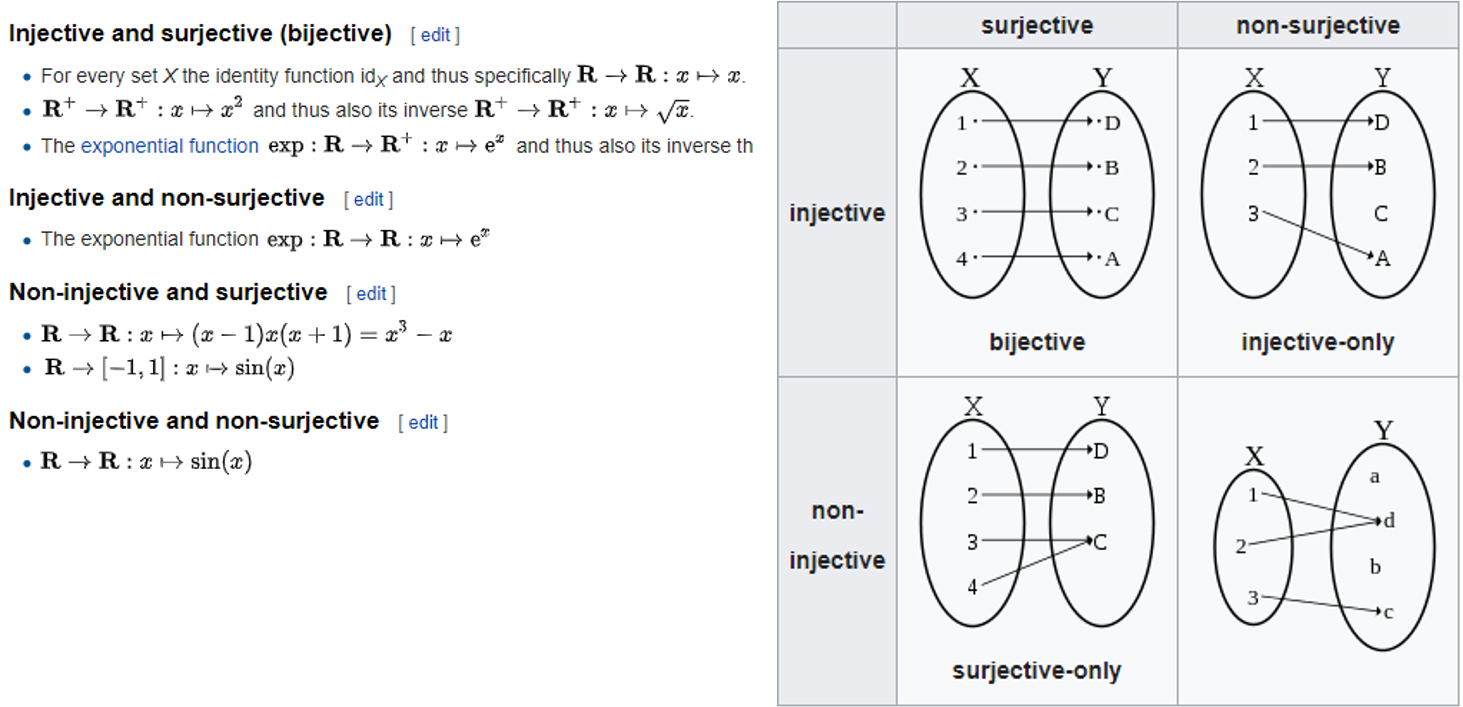
\includegraphics[height=6.5cm,width=1\textwidth,keepaspectratio]{bij_inj_surj_full.png}
%         \label{fig:bij_inj_surj_full.png}
%     \end{figure}
% \end{frame}

\begin{frame}[t]{Bijection, injection and surjection}
\framesubtitle{}
\vspace{-0.5cm}
\begin{columns}[T,onlytextwidth]
    \begin{column}{0.49\textwidth}
        \textbf{Injective and surjective (bijective)}\\
$\mathbf {R} \to \mathbf {R} :x\mapsto x.$

$\mathbf {R} ^{+}\to \mathbf {R} ^{+}:x\mapsto x^{2}$, and thus also its inverse $\mathbf {R} ^{+}\to \mathbf {R} ^{+}:x\mapsto {\sqrt {x}}.$.

\textbf{Injective and non-surjective}\\
$\mathbf {R} \to \mathbf {R} :x\mapsto \mathrm {e} ^{x}$.

\textbf{Non-injective and surjective}\\
$\mathbf {R} \to \mathbf {R} :x\mapsto (x-1)x(x+1)=x^{3}-x.$\\
$\mathbf {R} \to [-1,1]:x\mapsto \sin(x).$

\textbf{Non-injective and non-surjective}\\
$\mathbf {R} \to \mathbf {R} :x\mapsto \sin(x).$
    \end{column}
    \begin{column}{0.49\textwidth}
        \only<1>{
        \vspace{-0.4cm}
        \begin{figure}[H]
            \centering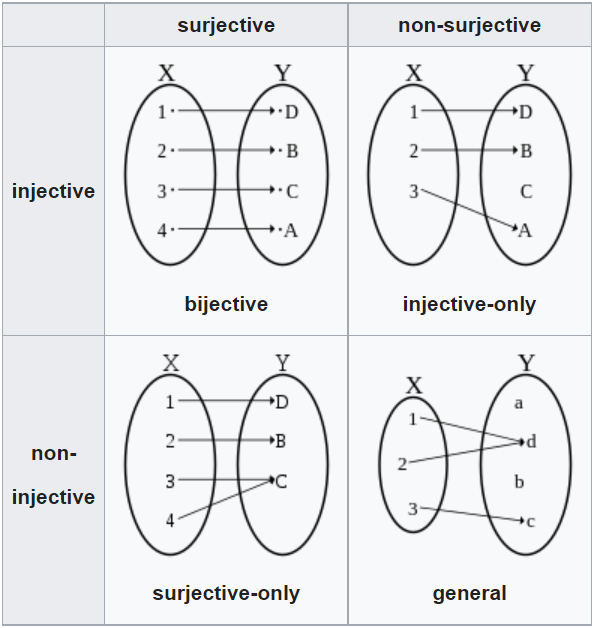
\includegraphics[height=6.5cm,width=1\textwidth,keepaspectratio]{bij_inj_surj.png}
            % \caption{caption_name}
            \label{fig:bij_inj_surj.png}
        \end{figure}
        }
    \only<2>{
        \begin{figure}[H]
            \begin{subfigure}{0.49\textwidth}
                \centering
                \resizebox{0.99\textwidth}{!}{
                \begin{tikzpicture}
                    \draw[->] (-1, 0) -- (3.2, 0) node[right] {$x$};
                    \draw[->] (0, -1) -- (0, 3.2) node[above] {$y$};
                    \draw[scale=1, domain=0:1.9, smooth, variable=\x, blue, ultra thick] plot ({\x}, {\x*\x}) node[right] {$f(x) =x^2$};
                    \draw[scale=1, domain=-1:3, smooth, variable=\y, red, ultra thick] plot ({\y}, {\y}) node[right] {$f(x) = x$};
                    \draw[scale=1, domain=0:3, smooth, variable=\z, green, ultra thick] plot ({\z}, {sqrt(\z)}) node[right] {$f(x) =\sqrt{x}$};
                  \end{tikzpicture}
                }
                \caption*{Bijective}
            \end{subfigure}
            \begin{subfigure}{0.49\textwidth}
                \centering
                \resizebox{0.89\textwidth}{!}{
                    \begin{tikzpicture}
                        \draw[->] (-2, 0) -- (2.5, 0) node[right] {$x$};
                        \draw[->] (0, -1) -- (0, 3.2) node[above] {$y$};
                        \draw[scale=1, domain=-2:1.2, smooth, variable=\x, blue, ultra thick] plot (\x,{exp(\x)}) node[right] {$f(x) =e^x$};
                    \end{tikzpicture}
                    }
                    \caption*{Injective-only}
            \end{subfigure}

            \begin{subfigure}{0.49\textwidth}
                \centering
                \resizebox{0.89\textwidth}{!}{
                    \begin{tikzpicture}
                        \draw[->] (-2, 0) -- (2.5, 0) node[right] {$x$};
                        \draw[->] (0, -1) -- (0, 2.2) node[above] {$y$};
                        \draw[scale=1, domain=-1.2:1.5, smooth, variable=\x, blue, ultra thick] plot (\x,{\x^3-\x}) node[right] {$f(x) =x^{3}-x$};
                        \draw[scale=1, domain=-1:1, smooth, variable=\y, red, ultra thick] plot (\y,{sin(\y r)}) node[right] {$f(x) =\sin(x)$};
                    \end{tikzpicture}
                    }
                    \caption*{Surjective-only}
            \end{subfigure}
            \begin{subfigure}{0.49\textwidth}
                \centering
                \resizebox{0.99\textwidth}{!}{
                \begin{tikzpicture}
                    \draw[->] (-3, 0) -- (3, 0) node[right] {$x$};
                    \draw[->] (0, -2) -- (0, 2) node[above] {$y$};
                    \draw[scale=1, domain=-2.8:2.8, smooth, variable=\x, blue, ultra thick] plot (\x,{sin(\x r)}) node[right] {$f(x) =\sin(x)$};
                  \end{tikzpicture}
                }
                \caption*{General}
            \end{subfigure}
        \end{figure}
    }
    \end{column}
\end{columns}
\end{frame}

\begin{frame}[t]{Task 4}
    \framesubtitle{}
    \only<1>{
        Transformation of a plane is given by $x^*=x^2-y^2$, $y^*=2xy$. Is this transformation an (a) injection; (b) surjection; (c) bijection? (d) Find the preimage of point $(x^*;y^*)$ by this transformation.
        }
    \only<2>{
        \alert{\Large Answer}
        
        (a): Not Injection \\ 
        (b): Is surjection \\ 
        (c): Not Bijection
    }
\end{frame}

\begin{frame}[t]{Affine Transformation}
\framesubtitle{In Computer Vision (CV)}
    \vspace{-0.6cm}
    \begin{figure}[H]
        \centering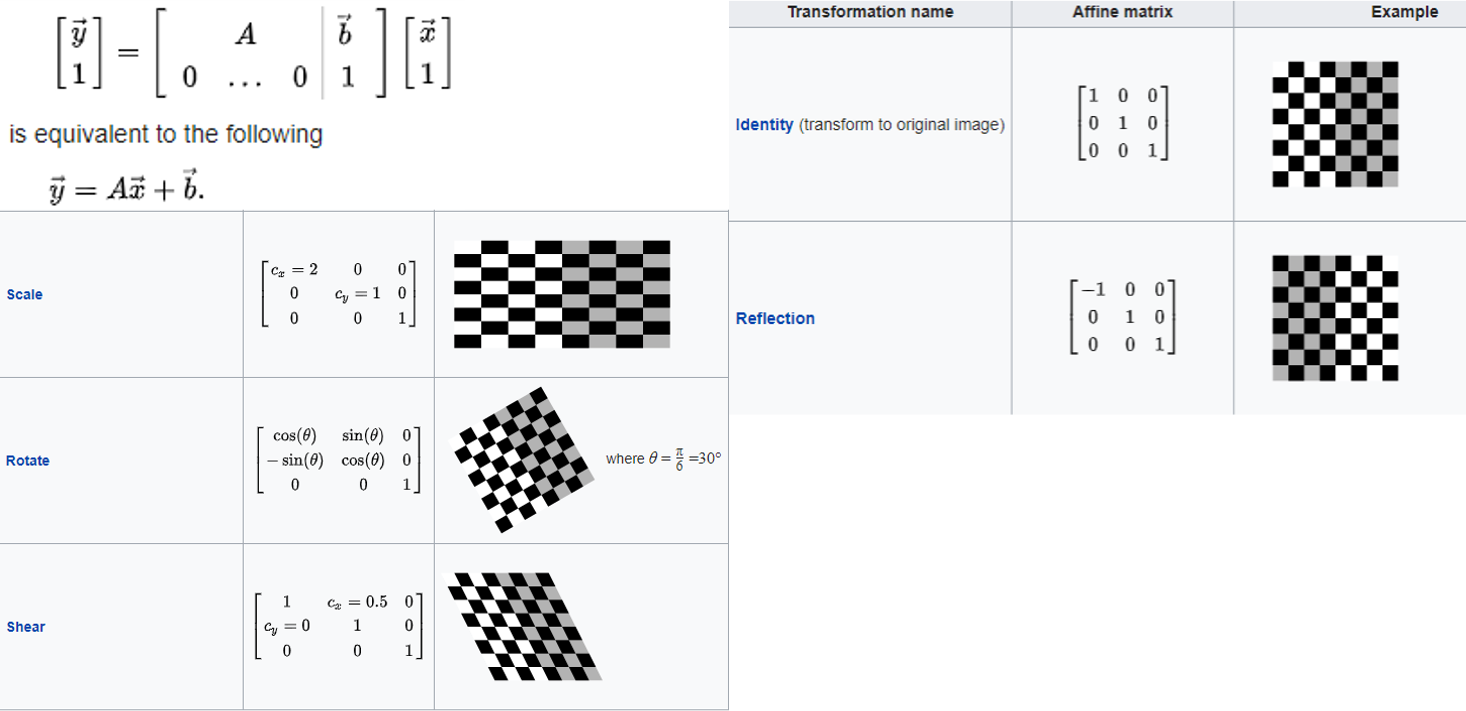
\includegraphics[height=6cm,width=1\textwidth,keepaspectratio]{affine_cv.png}
        \label{fig:affine_cv.png}
    \end{figure}
\end{frame}

\begin{frame}[t]{Affine Transformation}
    \framesubtitle{Video: intuition besides numbers 2D}
    \vspace{-0.6cm}
    \begin{figure}[H]
        \href{https://youtu.be/Y_TKQKdWC2k}{
            \centering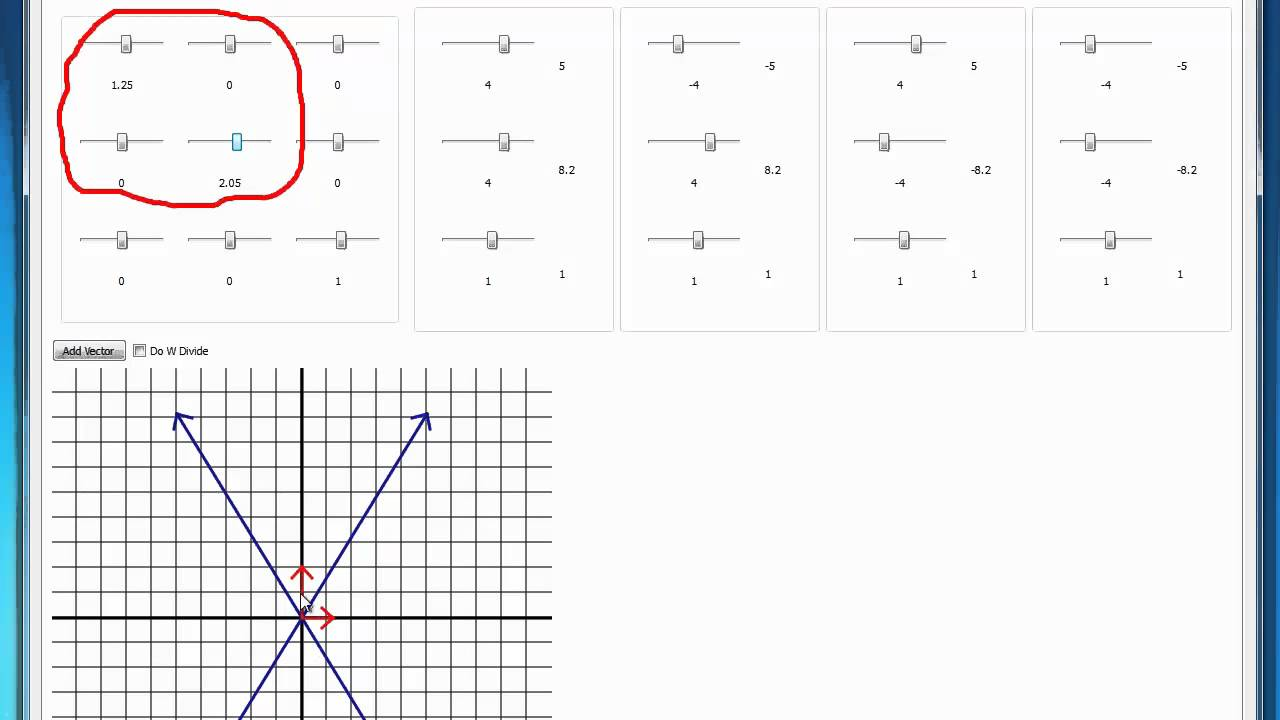
\includegraphics[height=6cm,width=1\textwidth,keepaspectratio]{num_intuition.jpg}}
        % \caption{Click on a picture for a video}
        \label{fig:num_intuition.jpg}
    \end{figure}
\end{frame}

\begin{frame}[t]{Affine Transformation}
    \framesubtitle{Video}
    \vspace{-0.6cm}
    \begin{figure}[H]
        \href{https://youtu.be/E3Phj6J287o}{
            \centering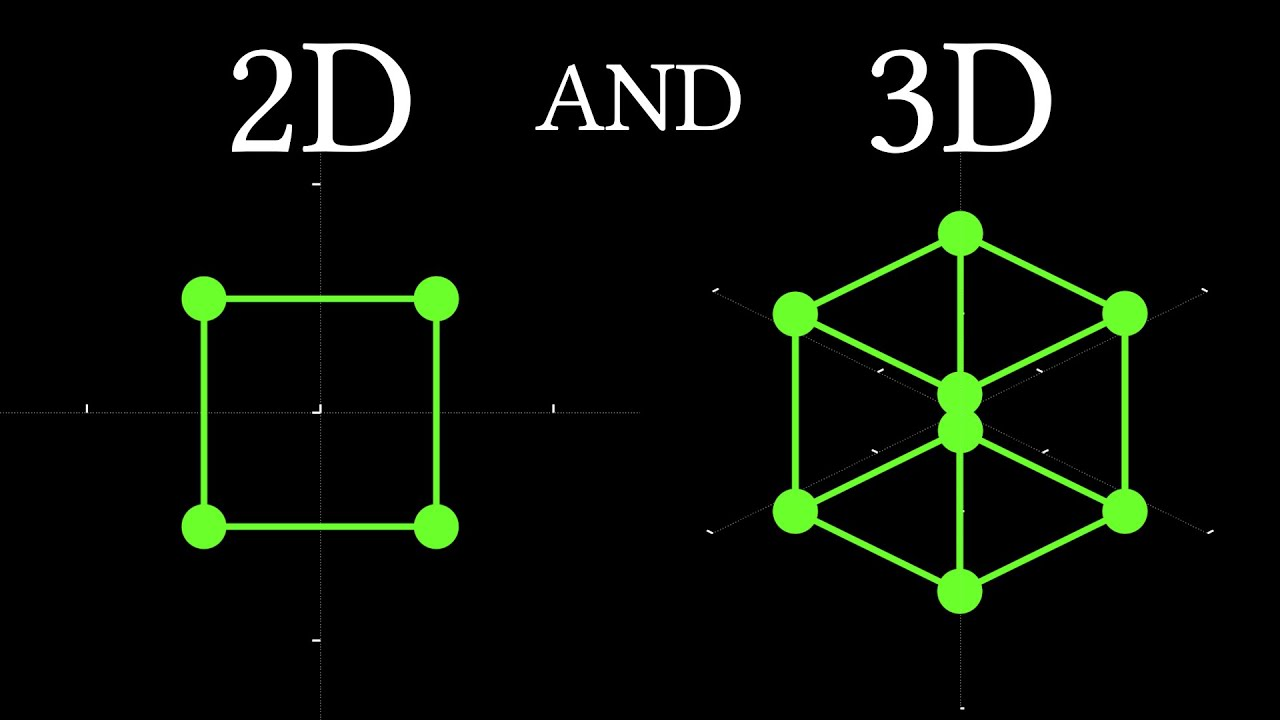
\includegraphics[height=6cm,width=1\textwidth,keepaspectratio]{num_intuition_3d.jpg}}
        % \caption{Click on a picture for a video}
        \label{fig:num_intuition_3d.jpg}
    \end{figure}
\end{frame}

\begin{frame}[t]{Affine Transformation}
    \framesubtitle{Application in CV (1)}
        \vspace{-0.6cm}
        \begin{figure}[H]
            \centering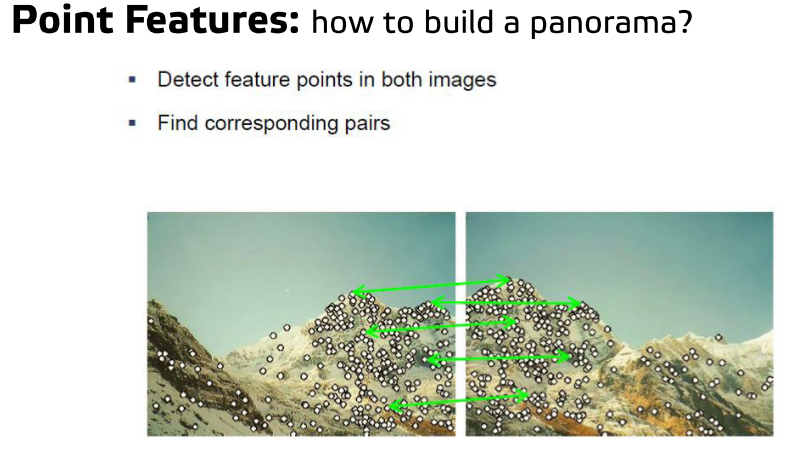
\includegraphics[height=6cm,width=1\textwidth,keepaspectratio]{cv_intro.png}
            \label{fig:cv_intro.png}
        \end{figure}
    \end{frame}

\begin{frame}[t]{Affine Transformation}
\framesubtitle{Application in CV (2)}
    \vspace{-0.6cm}
    \begin{figure}[H]
        \centering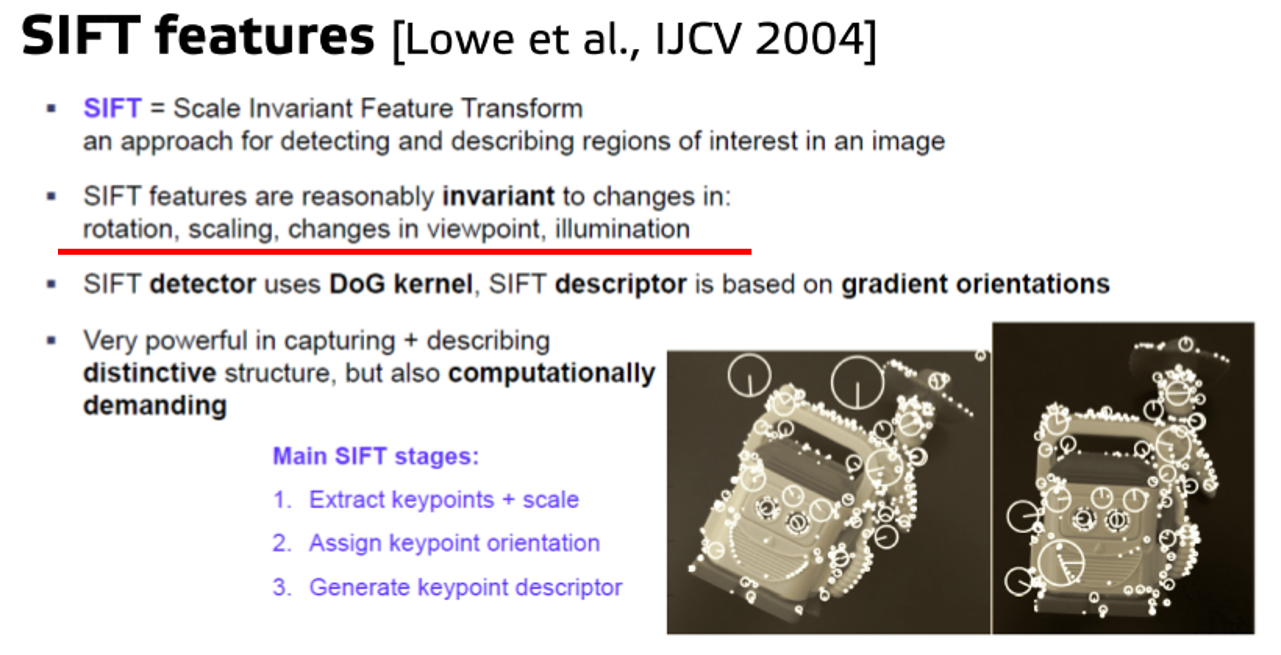
\includegraphics[height=6cm,width=1\textwidth,keepaspectratio]{sift.png}
        \label{fig:sift.png}
    \end{figure}
\end{frame}

\begin{frame}[t]{Affine Transformation}
    \framesubtitle{Application in CV (3)}
        \vspace{-0.6cm}
        \begin{figure}[H]
            \centering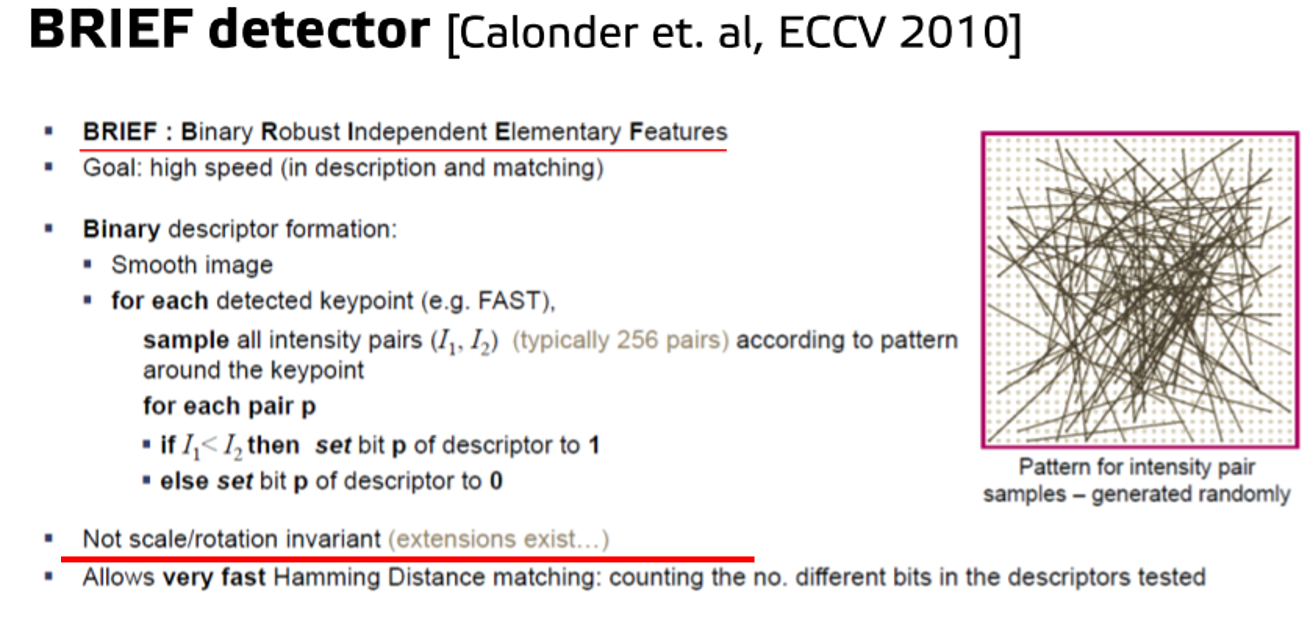
\includegraphics[height=6cm,width=1\textwidth,keepaspectratio]{brief.png}
            \label{fig:brief.png}
        \end{figure}
    \end{frame}

\begin{frame}[t]{Task 5}
    \framesubtitle{}
    \only<1>{
        Find the image of an arbitrary point $M$ which has position vector $\textbf{r}$ by the following transformations:

        (a) homothety with center $M_0(\textbf{r}_0)$ and ratio $\lambda\neq0$;
        
        (b) reflection across point $M_0(\textbf{r}_0)$;
        
        (c) translation by vector $\textbf{a}$;
        
        (d) orthogonal projection onto the line $\textbf{r}=\textbf{r}_0+\textbf{a}t$;
        
        (e) reflection across the line $\textbf{r}=\textbf{r}_0+\textbf{a}t$; 
        
        (f) dilation of factor $\lambda>0$ from the line $\textbf{r}=\textbf{r}_0+\textbf{a}t$.
        }
    \only<2>{
        \alert{\Large Answer}

        (a) $\textbf{r}^*=\textbf{r}_0+\lambda(\textbf{r}-\textbf{r}_0)$; 
        
        (b) $\textbf{r}^*=-\textbf{r}+2\textbf{r}_0$; 
        
        (c) $\textbf{r}^*=\textbf{r}+\textbf{a}$;
        
        (d) $\textbf{r}^*=\textbf{r}_0+\dfrac{\left(\textbf{r}-\textbf{r}_0\right)\cdot\textbf{a}}{|\textbf{a}|^2}\textbf{a}$; 
        
        (e) $\textbf{r}^*=2\textbf{r}_0-\textbf{r}+2\dfrac{\left(\textbf{r}-\textbf{r}_0\right)\cdot\textbf{a}}{|\textbf{a}|^2}\textbf{a}$;
        
        (f) $\textbf{r}^*=\lambda\textbf{r}+(1-\lambda)\textbf{r}_0+(1-\lambda) \dfrac{\left(\textbf{r}-\textbf{r}_0\right)\cdot\textbf{a}}{|\textbf{a}|^2}\textbf{a}$.
    }
\end{frame}

\begin{frame}[t]{Task 6}
    \framesubtitle{}
    \only<1>{
        Find formulas for the following affine transformations:

        (a) orthogonal projection onto line $x-3y+1=0$;
        
        (b) reflection across line $3x+4y-1=0$;
        
        (c) dilation from line $x+y-2=0$ of factor $\dfrac13$;
        
        (d) dilation from line $2x-y+5=0$ of factor 2.  
    }
    \only<2>{
        \alert{\Large Answer}

        (a) $x^*=\dfrac{9x+3y-1}{10}$, $y^*=\dfrac{3x+y+3}{10}$; 
        
        (b) $x^*=\dfrac{7x-24y+6}{25}$, $y^*={-24x-7y+8}{25}$; 
        
        (c) $x^*=\dfrac{2x-y+2}3$, $y^*=\dfrac{-x+2y+2}3$; 
        
        (d) $x^*=\dfrac{9x-2y+10}5$, $y^*=\dfrac{-2x+6y-5}5$.
    }
\end{frame}

\begin{frame}[t]{Task 7}
    \framesubtitle{}
    \only<1>{
    Find formulas for an affine mapping that transforms

(a) points $A(\dfrac37;\,1)$, $B(1;\dfrac14)$, $C(2;-1)$ into points $A^*(-4;\,2)$, $B^*(-1;\,6)$, $C^*(4;\,13)$ respectively;

(b) points $A(0;\,0)$, $B(-1;\,2)$, $C(1;-2)$ into points $A^*(-1;-1)$, $B^*(0;\,0)$, $C^*(1;\,1)$ respectively;

(c) points $A(2;\,0)$, $B(3;-1)$, $C(4;-2)$ into points $A^*(2;\,1)$, $B^*(-2;-1)$, $C^*(-6;-3)$ respectively;

(d) points $A(-2;\,0)$, $B(2;-1)$, $C(0;\,4)$ into points $A^*(-2;\,1)$, $B^*(2;\,1)$, $C^*(0;\,1)$ respectively.}
    \only<2>{
        \alert{\Large Answer}

        (a) $x^*=-4y$, $y^*=7x-1$; 
        
        (b) no solutions; 
        
        (c) $x^*=px+(p+4)y+2-2p$, $y^*=qx+(q+2)y+1-2q$, where $p$ and $q$ are any real numbers; 
        
        (d) no solutions (there exists a linear transformation that is not affine).
    }
\end{frame}

\begin{frame}[t]{Task 8}
    \framesubtitle{}
    Find all invariant lines of an affine transformation given by

(a) $x^*=y$, $y^*=1-x$;

(b) $x^*=2x+y-3$, $y^*=-3x-y$;

(c) $x^*=5x+3y+1$, $y^*=-3x-y$.

    \uncover<2->{
        \alert{\Large Answer}

        (a) no solutions; 
        
        (b) $x+y-3=0$, $2x-y+p=0$, where $p$ can be any real number; 
        
        (c) $x+y+1=0$.
    }
\end{frame}




\begin{frame}[t]{Reference material}
    % \framesubtitle{OnlineMschool}
    \Large
    \begin{itemize}
        \item \href{https://en.wikipedia.org/wiki/Bijection,_injection_and_surjection}{Bijection, injection and surjection (wiki)}
        \item \href{https://en.wikipedia.org/wiki/Affine_transformation}{Affine transformation (wiki)}
    \end{itemize}
\end{frame}

\fbckg{fibeamer/figs/last_page.png}
\frame[plain]{}

\end{document}